\documentclass[12pt]{extarticle}
\usepackage{ucs}
\usepackage[utf8x]{inputenc}
\usepackage{amsmath}
\usepackage{amssymb}
\usepackage{tikz}
\usepackage[unicode, pdftex]{hyperref}
\usepackage[russian]{babel}
\usepackage[T2A]{fontenc}
\usepackage{pgfplots}
\usepackage{amsthm}
\usepackage{latexsym}
\usepackage{mathtools}
\usepackage{listings}
\usepackage{color}
\usepackage{graphicx}
\usepackage{float}
\usepackage{wrapfig}
\title{Лингвистические нейросети, проходящие тест Тьюринга}
\author{Ларин Глеб}

\newtheorem*{remark}{Замечание}
\newtheorem{lemma}{Лемма}
\newtheorem*{definition}{Определение}
\newtheorem*{example}{Пример}


\lstset{ 
  belowcaptionskip=1\baselineskip,
  breaklines=true,
  frame=L,
  xleftmargin=\parindent,
  language=C++,
  showstringspaces=false,
  basicstyle=\footnotesize\ttfamily,
  keywordstyle=\bfseries\color{green!40!black},
  commentstyle=\itshape\color{purple!40!black},
  identifierstyle=\color{blue},
  stringstyle=\color{red},
}
	
\begin{document}


\maketitle
	Привет! Привет! Привет!!!!! Тут пока ничего нет, но скоро будет!
	. \newline
	.\newline
	.\newline
	.\newline
	.\newline
	
	\centerline{\textbf{I. Программирование математической состовляющей.}}
	\centerline{\textbf{Производные.}}
	Человек, благодаря развитому абстрактному мышлению, может представить себе бесконечность (в данном случае бесконечно малые), а от сюда и множественные математические идеи, которые строятся на ей. Одна из них - это производная. \newline
	
	Рассмотрим классическое определение производной:
	
	\centerline{$f'(x) = \displaystyle\lim_{\Delta x\to0} \frac{f(x+\Delta x) - f(x)}{\Delta x} $} 
	
	Благодаря формализации предела, человек может его понять, а как следствие, понять и производную. \newline
	
	Машина же не понимает слово стремится, потому что ей необходимы точные вычисления. В данном случае прибегнем к численному дифференцированию. 
	
	Убирая понятие предела, мы получаем:
	
	\centerline{$f'(x) = \frac{f(x+h) - f(x)}{h} $} 
	
	Где $h \rightarrow 0$ - шаг аппроксимации. \newpage
	Формулу (1.1) называют \textit{правой разностью} и аналогичным образом можно вывести формулу \textit{левой разности}:
	
	\centerline{$f'(x) = \frac{f(x) - f(x-h)}{h}$} 
	
	Чтобы найти ошибку правой и левой разности, разложим следующие функции в ряд Тейлора в точке x:
	
	\centerline{$f(x+h) = \displaystyle \sum_{k=0}^{n} \frac{f^{(k)}(x)}{k!}*(x+h-x)^k=\displaystyle \sum_{k=0}^{n} \frac{f^{(k)}(x)}{k!}*(h)^k$ (1.1)} 
	\centerline{$f(x-h) = \displaystyle \sum_{k=0}^{n} \frac{f^{(k)}(x)}{k!}*(x-h-x)^k=\displaystyle \sum_{k=0}^{n} \frac{f^{(k)}(x)}{k!}*(-h)^k$ (1.2)}
	
	Учитывая, что нам нужна только первая производная, то $n=1$. 
	
	\centerline{$f(x+h) = \displaystyle \sum_{k=0}^{1} \frac{f^{(k)}(x)}{k!}*(h)^k = f(x) + hf'(x) + \frac{R_1(x+h)}{h}$}
 	\centerline{$f(x-h) = \displaystyle \sum_{k=0}^{1} \frac{f^{(k)}(x)}{k!}*(-h)^k = f(x) - hf'(x) + \frac{R_1(x-h)}{h}$}
	
	Тогда:
	
	\centerline{$f'(x) = \frac{f(x+h) - f(x)}{h} + \frac{R_1(x+h)}{h} $} 
	\centerline{$f'(x) = \frac{f(x+h) - f(x)}{h} + \frac{R_1(x+h)}{h} $}
	
	Запишем же остаточный член в форме Лагранжа:
	
	\centerline{$R_1(x \pm h) = \frac{(x \pm h - x) ^ {1+1}}{(1+1)!} f^{(1+1)}[x+ \theta(x \pm h - x)] = \frac{h ^2}{2!} f''(x \pm \theta* h)$}
	\centerline{$\theta \in (0,1)$}
	
	Минимализируя шаг аппроксимации, получаем:
	
	\centerline{$\displaystyle \lim_{h \rightarrow 0} \theta h = 0$}
	
	Значит остаточный член, используя нотацию О-большого:
	
	\centerline{$R_1(x \pm h) = \frac{h ^2}{2} f''(x) = O(h^2) (1.3)$}
	
	Тогда погрешность левой и правой разности:
	
	\centerline{$f'(x) = \frac{f(x+h) - f(x)}{h} + \frac{O(h^2)}{h} = \frac{f(x+h) - f(x)}{h} + O(h)$} 
	\centerline{$f'(x) = \frac{f(x+h) - f(x)}{h} + \frac{O(h^2)}{h} =\frac{f(x+h) - f(x)}{h} +O(h)  $}
	
	\newpage
	Формулу (1.4) называют \textit{центральной разностью}. Именно её мы и будем использовать:
	
	\centerline{$f'(x) = \frac{f(x+h) - f(x-h)}{2h}$ (1.4)} 
	
	Чтобы найти её ошибку, вычтем из (1.2) формулу (1.1):
	
	\centerline{$f(x+h) - f(x-h) = 2*\displaystyle \sum_{k=0}^{n} \frac{f^{(2k+1)}(x)}{(2k+1)!}h^{2k+1}$}
	
	Поскольку нам нужна только первая производная, то $n = 1$:
	
	\centerline{$f(x+h) - f(x-h) = 2*\displaystyle \sum_{k=0}^{1} \frac{f^{(2k+1)}(x)}{(2k+1)!}h^{2k+1} + R_1(x+h) = 2(hf'(x) + R_2(x+h))$}
	
	\centerline{$\frac{f(x+h) - f(x-h)}{2} = hf'(x) + R_2(x+h)$}
	
	Аналогично выводу (1.3), получаем: \newline
	\centerline{$R_2(x+h) = \frac{f'''(x)}{3!}h^3 = O(h^3)$}
	
	Подставляя в центральную разность:
	
	\centerline{$\frac{f(x+h) - f(x-h)}{2} = hf'(x) + O(h^3)$}
	\centerline{$\frac{f(x+h) - f(x-h)}{2h} -  \frac{O(h^3)}{h} = f'(x)$}
	\centerline{$\frac{f(x+h) - f(x-h)}{2h} + {O(h^2)} = f'(x)$ (1.5)}
	
	Как мы видим, здесь ошибка много лучше, чем при использовании правой или левой разности. Конечно, мы можем продолжать раскладывать в ряд $f(x+2h)$, получая формулы двойной, четверной и прочих разностей, но тут вступает в силу погрешность вычисления компьютера. 
	
	Действительно, пусть $\epsilon \approx 10^{-16}$ - максимальная точность, которую может дать С++ (double). Полагая, что $\epsilon(x)\leq\epsilon$ - ошибка, которая получается при вычислении в точке х, мы получаем:
		
	\centerline{$\tilde{f}(x) = f(x) + \epsilon(x)$}
	\centerline{$\tilde{f}'(x) = f'(x) + \epsilon'(x)$} 
	 
	 
	\begin{remark}
		В данном контексте мы не рассматриваем ошибку аппроксимации, которая получилась в формулах выше.
	\end{remark}
	\centerline{$|\epsilon'(x)| = |\frac{\epsilon(x+h) - \epsilon(x)}{h}| \leq \frac{2\epsilon}{h}$}
	
	Таким образом, нетрудно вычислить и оптимальное h с учётом использования центральной разности, где ошибка аппроксимации $O(h^2)$:
	
	\centerline{$|f'(x) - \tilde{f}'(x)| = O(h^2) + \frac{2\epsilon}{h} $}
	
	Исходя из (1.3):
	
	\centerline{$O(h^2) = \frac{h^2}{2}f''(x)$}
	\centerline{$|f'(x) - \tilde{f}'(x)| = \frac{h^2}{2}f''(x) + \frac{2\epsilon}{h} $}
	
	Минимум же получается, если $\frac{h^2}{2}f''(x) = \frac{2\epsilon}{h}$, откуда h:
	
	\centerline{$h \approx \sqrt[3]{\frac{4\epsilon}{f''(x)}}$}
	
	Значит наилучший порядок оценки получается при $\sqrt[3]{\epsilon}$.
	
	Аналогично для любой из разностей, но для расчёта полной ошибки двойной разности, например, потребуются производные высших порядков, что вызывает затруднение, в отличии от двойной производной.
	
	Реализация этого на С++:
	
	\begin{lstlisting}
float approximation__devirate(function* __function, float __point_devirative,  float __derivative_step = APPROXIMATION_ORDER) {
    return ((*__function)(__point_devirative + __derivative_step) - (*__function)(__point_devirative - __derivative_step))/(2 * __derivative_step);
}
	\end{lstlisting}
						
	\centerline{\textbf{Частные производные и градиент.}}
	Для работы нейросетей необходимо запрограммировать возможность вычисления частных производных. Нам помогут выкладки, которые мы получили выше. 
	
	Пусть нам дана функция $f(x_1, x_2 \dots x_n)$. Исходя из определения частой производной в точке $(a_1, a_2 \dots a_n)$:
	
	\centerline{$ \frac{\partial f}{\partial x_i}(a_1, a_2 \dots a_n) = \displaystyle\lim_{\Delta x \rightarrow 0}\frac{f(a1 \dots a_i + \Delta x_i \dots a_n) - f(a_1, a_2 \dots a_n) } {\Delta x} $}
	
	Аналогично формуле (1.5) можно получить центральную разность для частных производных:
	
	\centerline{$\frac{f(a1 \dots a_i + h_i \dots a_n) - f(a1 \dots a_i - h_i \dots a_n)}{2h_i} + O(h_i^2) = \frac{\partial f}{\partial x_i}(a_1, a_2 \dots a_n)$ (1.6)}  
	
	Где $h_i \rightarrow 0$ - шаг аппроксимации при нахождении производной по i-ому аргументу функции. Учитывая, что все остальные аргументы принимаются за константу, то вывод $O(h_i^2)$ остаётся преждним. 
	
	Пользуясь формулой (1.6) можно легко численно посчитать градиент. 
	
	Пусть $\omega$ - функция от n переменных. Если же мы хотим вычислить градиент в точке $(a_1, a_2 .. a_n)$, то будет верна следующая формула:
	
	\centerline{$\nabla \omega(a_1, a_2 .. a_n) = (D_1\omega(a_1, a_2 .. a_n), \dots D_n\omega(a_1, a_2 .. a_n))$}
	\centerline{$D_i \omega = \frac{\partial \omega}{\partial x_i}$}
	
	\begin{remark}
		Здесь $\nabla$ - оператор набла. Учитывая, что градиент - это вектор, то он будет находиться в прямоугольной системе координат.
	\end{remark}
	
	\newpage
	Ошибка же вычисления градиента будет сумма ошибок всех вычислений частных производных с помощью центральной разности:
		
		\centerline{$\Theta = \displaystyle\sum_{i=0}^{n} O(h_i^2)$}
	
	Или же, если нам нужен вектор ошибки:
	
		\centerline{$\Theta_v = (O(h_1^2), O(h_2^2)... O(h_n^2))$}
		
	Где $O(h_i^2)$ вычисляется аналогично формуле (1.3):
	
		\centerline{$O(h_i^2) = \frac{h_i^2}{2} \frac{\partial^2 \omega}{\partial h_i^2}(a_1, a_2... a_n)$}
		
	Тогда градиент с учётом ошибки:
	
		\centerline{$\nabla \omega(a_1, a_2 .. a_n) = (D_1\omega(a_1, a_2 .. a_n), \dots D_n\omega(a_1, a_2 .. a_n)) + \Theta_v$}
	
	Реализация этого на С++:
	
		[Будет в дальнейшем]
		
	\centerline{\textbf{Матрицы.}}
		
		Кажется тривиальным, что для использования матриц подойдут двухмерные массивы или массив массивов. Да, это верно, но давайте рассмотрим обращение к таким объектам с помощью адрессной арифметики (рисунок один, так как для них будет одинаковое обращение):
		
	\begin{figure}[h]
			\centering
			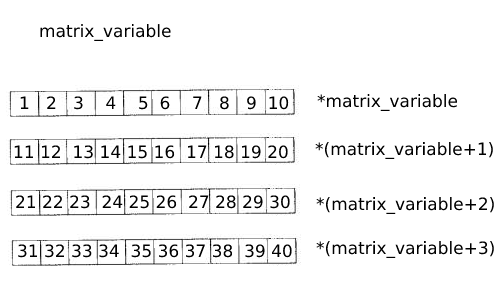
\includegraphics[width=0.8\linewidth]{matrix_1.png}
			\caption{Представление матрицы в виде двухмерного массива.}
			\label{fig:mpr}
	\end{figure}
	
	\newpage
	
	Чтобы получить какое-то $a_{ij}$, во-первых, необходимо получить его строку.
	
	Как мы видим, в памяти *\texttt{matrix\_variable} хранит массив, соответсвующий первой строке, *(\texttt{matrix\_variable}+1) - массив, соответсвующий второй строке и так далее.
	
	Чтобы получить уже элемент из нужного нам массива, опять обратимся к адресной арифметике:
	
	
	
	\begin{figure}[h]
			\centering
			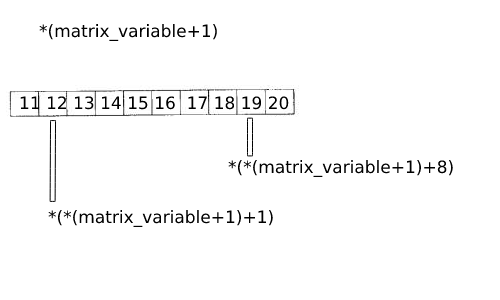
\includegraphics[width=0.8\linewidth]{matrix_2.png}
			\caption{Представление строки матрицы.}
			\label{fig:mpr}
	\end{figure}
	

	Получаем два указателя на один элемент. При работе с большими матрицами обращение через двойные указатели - это дорогая операция, а также зачастую неизвестно, куда ведёт такой двойной указатель: на следующую физическую ячейку, или на ячейку с каким-то случайным адресом - это остаётся проблемой. 
	Посчитаем количество тиков, которые занимает в таком случае обращение с помощью двойного указателя (рис 3).
	
	\begin{figure}[h]
			\centering
			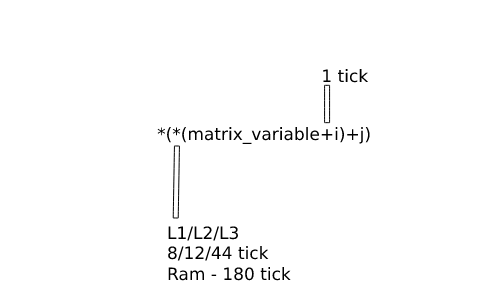
\includegraphics[width=0.8\linewidth]{matrix_3.png}
			\caption{Стоимость операций.}
			\label{fig:mpr}
	\end{figure}
	Исходя из \cite{litlink4} можно установить, что: 
	
	Стоимость сложения - 1 тик. 
	
	Стоимость обращения памяти зависит от того, куда попала наша переменная: в кэш, или в оперативную память, потому возьмём среднее значение - 61 тика.
	Суммарно вышло 124 тика.
	\newpage
	\begin{remark}
		На различных процессорах данные значения могут отличаться, потому мы взяли среднее значение. Также, у процессора есть несколько уровней кеширования, и на (рис 3) они обозначены L1, L2 и L3 соответственно.
	\end{remark} 
	
	Рассмотрим же другой способ представления матрицы: через одномерный массив. Исходя из (рис 4) легко понять работу такого метода: при объявлении матрицы он будет заполнять столбец, а после перейдёт на следующий. На (рис 4) массив будет представлен либо матрицой 2х5, либо 5х2.
	\begin{figure}[h]
			\centering
			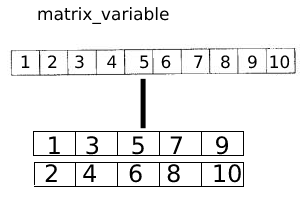
\includegraphics[width=0.4\linewidth]{matrix_4.png}
			\caption{Представление через одномерный массив.}
			\label{fig:mpr}
	\end{figure}
	
	\newpage
	
	\begin{remark}
		Фактически на линейном массиве мы организуем двойной.
	\end{remark}
	Теперь же разберёмся с обращением к такому массиву (рис 5).Чтобы получить какой-то элемент $a_{ij}$, мы будем применять формулу:
	
	\centerline{\texttt{*(matrix\_variable+N\_ROW*j+i)}}
	
	N\_ROW - количество строк в матрице. Может показаться, что таким образом мы будем хранить лишнее значение, которое добавит стоимость к операции обращения, но, во-первых, это значение нам заранее известно; во-вторых, в любом случае хранить размерность матриц необходимо для проверки при сложении и умножении, нахождении определителя.
	
	Посчитаем количество тиков в таком случае:
	
	Два сложения: 2 тика. 
	Одно умножение: 4 тика (среднее значение).
	Обращение к памяти: 61 тик. 
	
	Суммарно вышло 67 тиков, что быстрее более чем в полтора раза, чем двухмерный массив, потому вся дальнейшая реализация матриц будет строиться именно на одномерном массиве. 
		
	\begin{figure}[h]
			\centering
			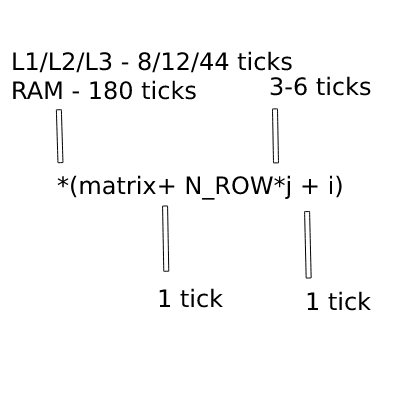
\includegraphics[width=0.4\linewidth]{matrix_5.png}
			\caption{Представление через одномерный массив.}
			\label{fig:mpr}
	\end{figure}
	
	
	\newpage
	
	
		\centerline{\textbf{II. Принцип работы нейросетей.}}
				\centerline{\textbf{Нейрон, активационная функция, индексация.}}
	Как и в мозге млекопитающих, за любое действие мозга отвечает нейрон, так и в любой нейросети за действие отвечает его имитация, которая принимает входные данные и выдаёт единственное значение, потому за каждый нейрон будет отвечать некоторая \textit{активационная} функция $\phi$.
	
	Учитывая её использование в дальнейших алгоритмах, то есть необходимое условие, чтобы $\phi$ нам подходила:

	\textit{1. Функция $\phi$ должна быть гладкой.} 
	
	\textit{2. Функция $\phi$ должна быть непрерывной.}
	
	\textit{3. $E(\phi) \in \mathbb{R} $}


	Теперь же необходимо понять, какие данные принимает функция активации нейрона.
	
	\begin{figure}[h]
			\centering
			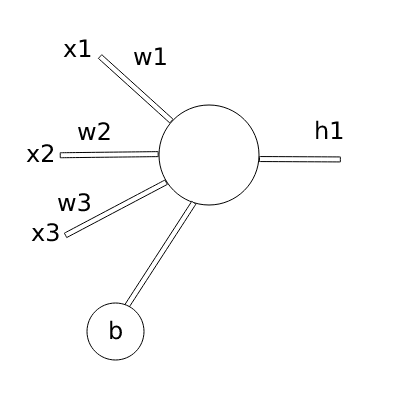
\includegraphics[width=0.4\linewidth]{neuron_1.png}
			\caption{Узел с несколькими входами.}
			\label{fig:mpr}
	\end{figure}
	
	
	На (рис 6) представлен узел. У каждого такого узла может быть больше входов, но каждый выход ведёт непросредственно в другой узел. Каждый вход и выход называется \textit{синапсом}. У каждого синапса есть некоторый коэффициент, называемый \textit{весом}. Система, состоящая из узла, синапса и активационной функции называется \textit{нейрон}.
	
	Вход же в активационную функцию рассчитывается следующей формулой:
	
	\centerline{$\displaystyle\sum_{i=0}^{n}x_iw_i + b $ (2.1)}
	
	В данном случае, n = 3 - количество входных синапсов, а b - коэффициент смещения. Он задерживает активацию нейрона (ниже будут представлены графики, где более подробно будет объяснено про роль коэффициента смещения).
	В таком случае выходной синапс нейрона:
	
	\centerline{$h_1 = \phi(\displaystyle\sum_{i=0}^{n}x_iw_i + b) $ (2.2)}
	В действительности современные нейросети содержат до нескольких миллардов нейронов \cite{litlink7}, из-за чего необходимо рассмотреть более сложную архитектуру:
	
	\begin{figure}[h]
			\centering
			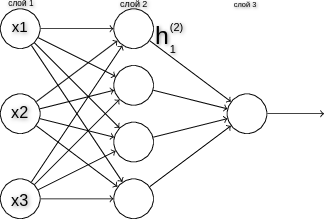
\includegraphics[width=0.7\linewidth]{neuron_2.png}
			\caption{Более комплексная система нейронов.}
			\label{fig:mpr}
	\end{figure}
	
	Слой, содержащий три нейрона (cлой 1), называется \textit{входным}, а содержащий один нейрон (слой 3) \textit{исходным}. Все слои, расположенные между этими двумя, называются \textit{скрытыми}.
	
	Так как каждые два нейрона содержат синапс, у каждого синапса свой вес, то необходимо ввести индексацию: $w_{ij}^{(l)}$
	
	i - номер узла в l+1 слое, а j - номер узла в l-ом слое (откуда-куда). Например $w_{21}^{(1)}$ означает вес синапса между вторый нейроном во втором слое и первым нейроном первого слоя.
	
	Аналогично для каждого нейрона есть коэффициент смещения, потому введём индексацию для него: $b_i^{(l)}$ - номер i-ого нейрона в l+1 слое.
	
	
	Выходное значение будем обозначать за $h_i^{(l)}$, где i - номер нейрона в l-ом слое.
	
	Выход исходного слоя обозначим $H$. 
	
	В таком случае перепишем (2.2) с учётом новой индексации:
	
	\centerline{$h_i^{l} = \displaystyle\phi(\sum_{k=0}^{n}w_{ik}^{(l-1)}x_k + b_i^{(l-1)})$ (2.3)}
	
	\centerline{\textbf{Процесс прямого распространения.}}
	
	\begin{remark}
		Все дальнейшие вычисления будут проводиться для системы нейронов, представленных на (рис 7), но они верны и для произвольной системы.
	\end{remark}
	
	Чтобы рассчитать H по заданным данным, мы воспользуемся формулой (2.3) и применим её для нашей системы на (рис 7):
	
	\centerline{$h_1^{(2)} = \phi(w_{11}^{(1)}x_1 + w_{12}^{(1)}x_2  + w_{13}^{(1)}x_3 + b_1^{(1)})$}
	\centerline{$h_2^{(2)} = \phi(w_{21}^{(1)}x_1 + w_{22}^{(1)}x_2  + w_{23}^{(1)}x_3 + b_2^{(1)})$}
	\centerline{$h_3^{(2)} = \phi(w_{31}^{(1)}x_1 + w_{32}^{(1)}x_2  + w_{33}^{(1)}x_3 + b_3^{(1)})$}
	\centerline{$H = h_1^{(3)} = \phi(w_{11}^{(2)}h_1^{(2)} + w_{12}^{(2)}h_2^{(2)}   + w_{13}^{(2)}h_3^{2} + b_1^{(2)})$}
	
	Для расчёта H вместо входных данных $x_i$ мы используем выходные данные от синапсов $h_i$. Аналогично будем делать, если в нашей системе несколько слоёв: выходный синапс одного нейрона является входным синапсом другого нейрона.
	
	Данная нотация прекрасно читается в случае малых размеров системы нейронов, но при большом их количестве, данная запись становится громодской, потому её можно записать через матрицы. 
	Чтобы не путаться с H, мы введём следующее обозначение:
	
	\centerline{ $\mathcal{H}^{(l)} = \begin{pmatrix}
		h_1^{(l)} \\
		\vdots \\
		h_n^{(l)}
	\end{pmatrix}$ (2.4)}
	
	В нашем случае же случае:
	
	\centerline{$\mathcal{H}^{(2)} = \begin{pmatrix}
		h_1^{(2)} \\
		h_2^{(2)} \\
		h_3^{(2)}
	\end{pmatrix}$}
	
	Немного изменим $\phi$: теперь она будет принимать матрицу и возвращать матрицу:
	
	\centerline{$\mathcal{H}^{(2)} = \begin{pmatrix}
		h_1^{(2)} \\
		h_2^{(2)} \\
		h_3^{(2)}
	\end{pmatrix} = \phi\begin{pmatrix}
		w_{11}^{(1)}x_1 + w_{12}^{(1)}x_2  + w_{13}^{(1)}x_3 + b_1^{(1)} \\
		w_{21}^{(1)}x_1 + w_{22}^{(1)}x_2  + w_{23}^{(1)}x_3 + b_2^{(1)} \\
		w_{31}^{(1)}x_1 + w_{32}^{(1)}x_2  + w_{33}^{(1)}x_3 + b_3^{(1)} \end{pmatrix}$}
	\newpage
	Поподробнее рассмотрим матрицу, которая является агрументом:
	
	\centerline{$\begin{pmatrix}
		w_{11}^{(1)}x_1 + w_{12}^{(1)}x_2  + w_{13}^{(1)}x_3 + b_1^{(1)} \\
		w_{21}^{(1)}x_1 + w_{22}^{(1)}x_2  + w_{23}^{(1)}x_3 + b_2^{(1)} \\
		w_{31}^{(1)}x_1 + w_{32}^{(1)}x_2  + w_{33}^{(1)}x_3 + b_3^{(1)} \end{pmatrix} = \begin{pmatrix}
		w_{11}^{(1)}x_1 + w_{12}^{(1)}x_2  + w_{13}^{(1)}x_3  \\
		w_{21}^{(1)}x_1 + w_{22}^{(1)}x_2  + w_{23}^{(1)}x_3  \\
		w_{31}^{(1)}x_1 + w_{32}^{(1)}x_2  + w_{33}^{(1)}x_3 \end{pmatrix} +\begin{pmatrix}
		b_1^{(1)} \\
		b_2^{(1)} \\
		b_3^{(1)} \end{pmatrix} $}
	
	\centerline{$\begin{pmatrix}
		w_{11}^{(1)}x_1 + w_{12}^{(1)}x_2  + w_{13}^{(1)}x_3  \\
		w_{21}^{(1)}x_1 + w_{22}^{(1)}x_2  + w_{23}^{(1)}x_3  \\
		w_{31}^{(1)}x_1 + w_{32}^{(1)}x_2  + w_{33}^{(1)}x_3 \end{pmatrix} +\begin{pmatrix}
		b_1^{(1)} \\
		b_2^{(1)} \\
		b_3^{(1)} \end{pmatrix} = \begin{pmatrix}
		w_{11}^{(1)} & w_{12}^{(1)} & w_{13}^{(1)}  \\
		w_{21}^{(1)} & w_{22}^{(1)} & w_{23}^{(1)}  \\
		w_{31}^{(1)} & w_{32}^{(1)} & w_{33}^{(1)} \end{pmatrix} * \begin{pmatrix}
		x_1  \\
		x_2\\
		x_3 \end{pmatrix} +\begin{pmatrix}
		b_1^{(1)} \\
		b_2^{(1)} \\
		b_3^{(1)} \end{pmatrix} $}
		
		Как мы видим, наша матрица является композицией нескольких: матрицы весов, входных синапсов и коэффициентов смещения. 
		
		
		Положим следующее:
		
		\centerline{$\mathcal{B}^{(l)} = \begin{pmatrix}
		b_1^{(l)} \\
		\vdots \\
		b_n^{(l)} \end{pmatrix} $}
		
		\centerline{$\mathcal{W}^{(l)} = \begin{pmatrix}
		w_{11}^{(l)} & \cdots & w_{1i}^{(l)} \\ 
		\vdots & \ddots & \vdots \\
		w_{j1}^{(l)} & \dots & w_{ji}^{(l)} \end{pmatrix}$}
		
	Тогда наш выходной слой в новых обозначениях:
	
	\centerline{$\mathcal{H}^{(2)} =\phi(\mathcal{W}^{(1)} * \mathcal{H}^{(1)} +  \mathcal{B}^{(1)})$}
	
	\begin{remark}
		$\mathcal{H}_1$ - матрица входных значений нейросети.
	\end{remark}
	
	Исходя из этого:
	
	\centerline{$H = \mathcal{H}^{(3)} = \phi(\mathcal{W}^{(2)} * \mathcal{H}^{(2)} +  \mathcal{B}^{(2)})$}
	
	В дальнейшем будет пользоваться этим в общем виде:
	
	\centerline{$\mathcal{H}^{(l)} =  \phi(\mathcal{W}^{(l-1)} * \mathcal{H}^{(l-1)}+  \mathcal{B}^{(l-1)})$}
	\newpage	
\addcontentsline{toc}{section}{Список используемой литературы}
 
\begin{thebibliography}{}
    \bibitem{litlink1} В. А. Зорич, "Математический анализ .Часть I"\ , 10-ое издание

    \bibitem{litlink2}  Н.С.Бахвалов, Н.П.Жидков, Г.М.Кобельков,
"Численные методы"\ , учебное пособие

    \bibitem{litlink3} Р.З. Даутов, М.М. Карчевский, "Основы численных методов линейной алгебры"\ , учебное пособие
    
    \bibitem{litlink4} Agner Fog, “Instruction tables. Lists of instruction latencies, throughputs and micro-operation breakdowns for Intel, AMD and VIA CPUs”\ , стр 296-312 \newline
    
    \bibitem{litlink5} 
    
    \bibitem{litlink6} Loc Vu-Quoc, Alexander Hume, "Deep learning applied to computational mechanics: A comprehensive review, state of the art, and the classics"
    \bibitem{litlink7} Andrew Trask, David Gilmore, Matthew Russell, "Modeling Order in Neural Word Embeddings at Scale"\ - стр 8
    
\end{thebibliography}
\end{document}

